 \section[Physics of Semiconductors (and metals and insulators)]{\hyperlink{toc}{Physics of Semiconductors (and metals and insulators)}}


- InSb is the smallest bandgap in the III-V semiconductor group


\textbf{Metals:}

- Light will excite electrons, free to move and reemit light so they look shiny.
- Conduction band width determines solver, gold, copper colour etc,

\textbf{Impurities:}

- crystal colour is effected by impurities such as Nitrogen in Diamond making it look yellow or Boron impurity making it look blue.

(area of research -- \textbf{Nitrogen-Vacancy center in diamond})

- or oxides (insulator) on shiny metal (conductor) can make it look matte.

\textbf{Basic Properties of Semiconductors}


\textbf{Electrons and Holes:}
\begin{itemize}
    \item semiconductor with filled VB and excite one electron to the conduction band (photon absorption or thermal excitation).
    \item \textbf{Hole} is then the absence of an electron in VB.
\end{itemize}

 
 \begin{figure}
 \centering
  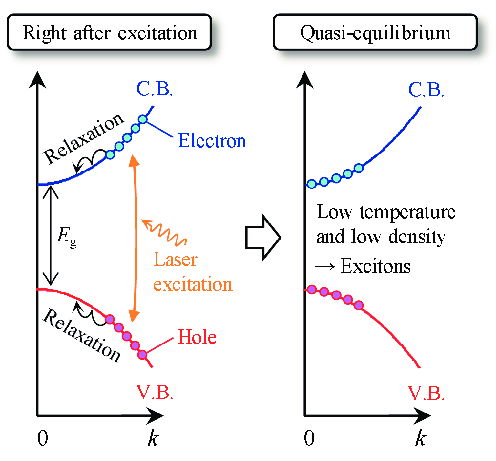
\includegraphics[width=0.75\linewidth]{Images/electron-holes.png}
  \caption{electronholes}
  \label{fig:electronholes}
\end{figure}

\textbf{Holes}
\begin{itemize}
    \item convenient to keep track of the holes 
    \item effectively act like a positive charge
    \item moves like a particle
    \item has charge and mass
    \item not a real particle $\xrightarrow{}$ only a quasi-particle
    \item electrons here with effective mass are actually also quasi-particles
    \item electron and hole pair attract each other and for another quasi-particle called an exciton
    \item exciton is a Boson because it is composed of two Fermions (electon and holes). (bose-einstein condensate is a field of research that is not covered in the course).
    \item electron can fall back, "annihilating" the conduction electron and the hole in the valence band (analogous to electron-positron, particle-antiparticle pair).
    \item convention to make mass of hole positive, since it takes energy to accelerate the hole from zero vel to finite vel (like pushing a balloon underwater).
\end{itemize}


\begin{equation}
    \frac{\hbar^2}{m_h^*} = -\frac{\partial ^2E}{\partial k^2} = 2 \alpha
\end{equation}

\textbf{How to Measure the Effective Mass}

- Cyclotron Resonance Technique
\[F = \frac{mv^2}{r} = qvB\]

\[ f = \frac{qB}{2\pi m} \]

- independent or v and r 

- electrons strongly absorb microwaves of that frequency

- only need to measure freq to solve for effective mass.



\begin{tabular}{ |p{1.5cm}|p{1.5cm}|p{1.5cm}|p{1.5cm}|p{1.5cm}|p{1.5cm}|  }
 \hline
 \multicolumn{6}{|c|}{\textbf{Electron and hole effective masses}} \\
 \hline
    & Si & Ge & GaAs & InAs & AlAs\\
 \hline
 $m_n/m_0$ & 0.26 & 0.12 & 0.068 & 0.023 & 2 \\
 $m_p/m_0$ & 0.39 & 0.3 & 0.5 & 0.3 & 0.3 \\
 \hline
\end{tabular}

\textbf{Doping Semiconductors}
\begin{itemize}
    \item pure ins. or semcond. excite electrons from VB to CB and the density of electrons in the conduction band (n for negative charges) is equal to the density of holes in the valence band (p for positive charges).
    \item \textbf{Intrinsic:} semiconductor without impurities
    \item \textbf{Extrinsic:} when impurities are placed in the SC
\end{itemize}



\textbf{Intrinsic Carrier Concentration:}

\begin{itemize}
    \item Density of States (DoS): how many eigenstates at each energy. 
\end{itemize}

 \begin{tcolorbox}[enhanced,attach boxed title to top center={yshift=-3mm,yshifttext=-1mm},
  colback=blue!5!white,colframe=blue!75!black,colbacktitle=red!80!black,
  title=Law of Mass Action,fonttitle=\bfseries,
  boxed title style={size=small,colframe=red!50!black} ]
  \begin{equation}
      np = 4\left(\frac{1}{2\pi\hbar^2\beta}\right)^3(m_em_h)^{3/2}e^{-\beta E_g}
  \end{equation}
\end{tcolorbox}

 intrinsic carrier concentration -- Fermi level is inside the gap and the density of holes and electrons are equal then each density is the sqrt of the above expression on the right.
 
 
 It is often useful to intentionally add impurities.
 
 Consider:
 \begin{itemize}
     \item silicon a semiconductor with a bandgap of 1.1eV
     \item replace one atom with phosphorus (which has one extra proton and one extra electron)
     \item VB is filled and so electron must go into the conduction band
     \item known as donor, \textbf{electron donor}, or \textbf{n-dopant}, as n is the symbol from the density of electrons in the conduction band.
 \end{itemize}
 
 or instead:
 \begin{itemize}
     \item replace one atom with Aluminium
     \item provides one fewer electron than silicon
     \item missing electron from the VB, leaving a hole.
     \item known as \textbf{electron acceptor}, or a \textbf{p-dopant}
 \end{itemize}
 
 - semiconductor Fermi energy is in the middle of the band gap, and then dopants shift it up for n-dopant case and down for the p-dopant case. 
